\documentclass[12pt,a4paper]{article}
\usepackage[margin=2.5cm]{geometry}
\usepackage{amsmath,amssymb,amsfonts}
\usepackage{physics}
\usepackage{enumitem}
\usepackage{fancyhdr}
\usepackage{lastpage}
\usepackage{graphicx}
\usepackage{multicol}
\usepackage{array}
\usepackage{tabularx}
\usepackage{tikz}
\usepackage{xcolor}
\usepackage{tcolorbox}

% Page style
\pagestyle{fancy}
\fancyhf{}
\renewcommand{\headrulewidth}{0.4pt}
\renewcommand{\footrulewidth}{0.4pt}
\lhead{PHYS10012}
\rhead{Mock Examination --- Solutions}
\cfoot{Page \thepage\ of \pageref{LastPage}}

% Question numbering
\newcounter{questioncounter}
\newcommand{\question}[1]{%
  \stepcounter{questioncounter}%
  \vspace{0.5cm}%
  \noindent\textbf{Question \thequestioncounter.} \hfill [#1 marks]%
  \vspace{0.2cm}%
  \par%
}

% Sub-part environments
\newlist{parts}{enumerate}{2}
\setlist[parts,1]{label=(\alph*),leftmargin=2em,itemsep=0.3cm}
\setlist[parts,2]{label=(\roman*),leftmargin=2em,itemsep=0.2cm}

% Mark allocation
\renewcommand{\marks}[1]{\hfill [#1]}
\newcommand{\markstep}[1]{\hfill\textcolor{blue}{[#1]}}

% Boxed final answer
\newcommand{\finalanswer}[1]{%
  \begin{tcolorbox}[colback=green!5!white,colframe=green!50!black,boxrule=0.5pt]
  #1
  \end{tcolorbox}
}

% Equation source notation
\newcommand{\fromsheet}{\textit{(From formula sheet)}}
\newcommand{\recalled}{\textit{(Recalled --- not on formula sheet)}}

% MCQ answer format
\newcounter{mcqcounter}
\newcommand{\mcqanswer}[2]{%
  \stepcounter{mcqcounter}%
  \noindent\textbf{\themcqcounter.} \textbf{#1} --- #2\\[0.2cm]%
}

% Dirac notation shortcuts
\renewcommand{\ket}[1]{\left|#1\right\rangle}
\renewcommand{\bra}[1]{\left\langle #1\right|}
\renewcommand{\braket}[2]{\left\langle #1\middle|#2\right\rangle}
\renewcommand{\ketbra}[2]{\left|#1\right\rangle\!\left\langle #2\right|}
\renewcommand{\expect}[1]{\left\langle #1\right\rangle}

\begin{document}

% Title block
\begin{center}
{\Large\textbf{UNIVERSITY OF BRISTOL}}\\[0.3cm]
{\large Faculty of Science}\\[0.5cm]
{\Large\textbf{MOCK EXAMINATION --- Paper 6 (Easy) --- SOLUTIONS AND MARK SCHEME}}\\[0.3cm]
{\large\textbf{Core Physics I --- Classical, Quantum and Thermal Physics}}\\[0.2cm]
{\large Module Code: PHYS10012}\\[0.5cm]
{\large Total Marks: 100}\\[0.3cm]
\end{center}

\noindent\rule{\textwidth}{0.4pt}

\vspace{0.3cm}
\noindent\textbf{Marking Notes:}
\begin{itemize}[itemsep=0.1cm]
\item Mark allocations are shown in \textcolor{blue}{blue} at each step.
\item Final answers are highlighted in green boxes.
\item ``\fromsheet'' indicates the equation is on the provided formula sheet.
\item ``\recalled'' indicates the equation must be known from memory.
\item Award partial marks for correct method even if the final answer is wrong.
\item Accept equivalent correct forms of answers.
\end{itemize}

\noindent\rule{\textwidth}{0.4pt}
\newpage

% ============================================================
% SECTION A: OSCILLATIONS AND WAVES MCQ ANSWERS
% ============================================================
\section*{Section A: Oscillations and Waves --- Answers}

\setcounter{mcqcounter}{0}

\mcqanswer{B}{Simple harmonic motion is defined by a restoring force that is directly proportional to the displacement from equilibrium and directed toward the equilibrium position: $F = -kx$. This linear restoring force is the defining property of SHM.}

\mcqanswer{C}{The period of a mass--spring system is $T = 2\pi\sqrt{m/k}$ \fromsheet. With $m = 0.5\;\text{kg}$ and $k = 200\;\text{N/m}$: $T = 2\pi\sqrt{0.5/200} = 2\pi\sqrt{0.0025} = 2\pi\times 0.05 = 0.314\;\text{s}$.}

\mcqanswer{B}{The maximum speed in SHM is $v_{\max} = A\omega_0$ \recalled. With $A = 0.10\;\text{m}$ and $\omega_0 = 5\;\text{rad/s}$: $v_{\max} = 0.10\times 5 = 0.50\;\text{m/s}$.}

\mcqanswer{B}{The quality factor is defined as $Q = \omega_0/\gamma$ \fromsheet, the ratio of the natural angular frequency to the damping constant.}

\mcqanswer{B}{The wave speed is $v = f\lambda$ \recalled. With $f = 500\;\text{Hz}$ and $\lambda = 0.68\;\text{m}$: $v = 500\times 0.68 = 340\;\text{m/s}$.}

\mcqanswer{C}{In the $n$th harmonic of a string fixed at both ends, there are $n$ antinodes (and $n+1$ nodes). For the 3rd harmonic, there are 3 antinodes.}

\mcqanswer{C}{The decibel formula is $\beta = 10\log_{10}(I/I_0)$ \fromsheet, where $I_0 = 10^{-12}\;\text{W/m}^2$ is the reference intensity. At $\beta = 0\;\text{dB}$: $0 = 10\log_{10}(I/I_0)$, so $I/I_0 = 1$, giving $I = I_0 = 10^{-12}\;\text{W/m}^2$.}

\mcqanswer{C}{When a source moves toward an observer, the effective wavelength is compressed (shorter), resulting in a higher observed frequency. From the Doppler formula $f' = f\,v/(v - v_s)$ \fromsheet, with $v_s > 0$ (approaching), the denominator is less than $v$, so $f' > f$.}

\mcqanswer{B}{The beat frequency is $f_{\text{beat}} = |f_1 - f_2|$ \recalled. With $f_1 = 256\;\text{Hz}$ and $f_2 = 260\;\text{Hz}$: $f_{\text{beat}} = |256 - 260| = 4\;\text{Hz}$.}

\mcqanswer{B}{The period of a simple pendulum is $T = 2\pi\sqrt{L/g}$ \fromsheet. It depends only on the length $L$ of the string and the acceleration due to gravity $g$, not on the mass of the bob or the amplitude (for small oscillations).}

\newpage

% ============================================================
% SECTION B: QUANTUM PHYSICS MCQ ANSWERS
% ============================================================
\section*{Section B: Quantum Physics --- Answers}

\setcounter{mcqcounter}{0}

\mcqanswer{C}{The symbol $\ket{\psi}$ is a ket, which represents a quantum state (state vector) in a Hilbert space. It is not a number, a probability, or an operator.}

\mcqanswer{D}{The inner product $\braket{\phi}{\psi}$ is a complex scalar (a complex number). It is the ``overlap'' between the two states. \recalled}

\mcqanswer{B}{By the Born rule, $|\braket{\phi}{\psi}|^2$ gives the probability of finding the system in state $\ket{\phi}$ given it is in state $\ket{\psi}$ (or equivalently, the transition/overlap probability). \recalled}

\mcqanswer{C}{In the eigenvalue equation $\hat{A}\ket{a} = a\ket{a}$, the scalar $a$ is called the eigenvalue (and $\ket{a}$ is the eigenvector or eigenstate). \recalled}

\mcqanswer{B}{For a spin-$\frac{1}{2}$ particle, the eigenvalues of $S_z$ are $+\hbar/2$ (spin up) and $-\hbar/2$ (spin down). These follow from $S_z = \frac{\hbar}{2}\sigma_z$ \fromsheet.}

\mcqanswer{C}{The normalisation condition requires $\braket{\psi}{\psi} = |\alpha|^2 + |\beta|^2 = 1$ \recalled. Note the modulus squared, not the square of the coefficients (since $\alpha$ and $\beta$ may be complex).}

\mcqanswer{C}{An operator is Hermitian (self-adjoint) if $\hat{A}^\dagger = \hat{A}$. This ensures its eigenvalues are real, which is required for physical observables. \recalled}

\mcqanswer{C}{For spin quantum number $s$, the number of distinct spin states is $2s + 1$. For $s = 1$: $2(1) + 1 = 3$ states, corresponding to $m_s = -1, 0, +1$.}

\mcqanswer{C}{The proton ($uud$) has charge $+\frac{2}{3}e + \frac{2}{3}e - \frac{1}{3}e = +\frac{4}{3}e - \frac{1}{3}e = +1e = +e$. \recalled}

\mcqanswer{B}{An electron is a fermion (it has spin-$\frac{1}{2}$) and a lepton (it is a fundamental particle in the lepton family, not composed of quarks). \recalled}

\newpage

% ============================================================
% SECTION C: LONG ANSWER SOLUTIONS
% ============================================================
\section*{Section C: Long Answer Solutions}

\setcounter{questioncounter}{0}

% ---- SOLUTION C1: MECHANICS (15 marks) ----
\question{15}

\noindent\textbf{SUVAT, Forces, and Energy --- Direct Application}

\begin{parts}

%% (a) Projectile — vertical throw [3 marks]
\item

\textbf{(i)} At maximum height, $v = 0$. Using $v = u + at$ with $u = 20\;\text{m/s}$, $a = -g = -9.81\;\text{m/s}^2$: \fromsheet

$0 = 20 - 9.81\,t$

\finalanswer{$t = \dfrac{20}{9.81} = 2.04\;\text{s}$} \markstep{1}

\textbf{(ii)} Using $v^2 = u^2 + 2as$ with $v = 0$: \fromsheet

$0 = 20^2 + 2(-9.81)h$

$h = \dfrac{400}{2\times 9.81} = \dfrac{400}{19.62}$

\finalanswer{$h = 20.4\;\text{m}$} \markstep{1}

\textbf{(iii)} By symmetry, the total time of flight is twice the time to reach maximum height:

\finalanswer{$t_{\text{total}} = 2\times 2.04 = 4.08\;\text{s}$} \markstep{1}

(Alternatively, use $s = ut + \frac{1}{2}at^2$ with $s = 0$: $0 = 20t - \frac{1}{2}(9.81)t^2$, giving $t(20 - 4.905t) = 0$, so $t = 0$ or $t = 20/4.905 = 4.08\;\text{s}$.)

%% (b) Box with friction [3 marks]
\item

\textbf{(i)} Forces acting on the $10\;\text{kg}$ box: \markstep{1}
\begin{itemize}
\item Weight $W = mg = 10\times 9.81 = 98.1\;\text{N}$ downward.
\item Normal force $N = 98.1\;\text{N}$ upward (balances weight on horizontal surface).
\item Applied force $F = 60\;\text{N}$ horizontal, in the direction of motion.
\item Kinetic friction $f_k$ opposing the motion (horizontal, opposite to applied force).
\end{itemize}

\textbf{(ii)} The kinetic friction force is: \recalled

$f_k = \mu_k N = \mu_k mg = 0.4\times 10\times 9.81$

\finalanswer{$f_k = 39.2\;\text{N}$} \markstep{1}

\textbf{(iii)} Applying Newton's second law ($F_{\text{net}} = ma$) horizontally: \recalled

$F - f_k = ma$

$60 - 39.2 = 10\,a$

$a = \dfrac{20.8}{10}$

\finalanswer{$a = 2.08\;\text{m/s}^2$} \markstep{1}

%% (c) Energy conservation with spring [4 marks]
\item

\textbf{(i)} Using conservation of energy for the ball falling from height $h = 5\;\text{m}$: \recalled

$mgh = \tfrac{1}{2}mv^2$

$v = \sqrt{2gh} = \sqrt{2\times 9.81\times 5} = \sqrt{98.1}$ \markstep{1}

\finalanswer{$v = 9.90\;\text{m/s}$} \markstep{1}

\textbf{(ii)} The ball slides onto the frictionless horizontal surface at speed $v = 9.90\;\text{m/s}$ and compresses the spring. At maximum compression $x$, all kinetic energy is stored as elastic potential energy: \recalled

$\tfrac{1}{2}mv^2 = \tfrac{1}{2}kx^2$ \markstep{1}

$x = v\sqrt{\frac{m}{k}} = 9.90\times\sqrt{\frac{2}{500}} = 9.90\times\sqrt{0.004} = 9.90\times 0.06325$

\finalanswer{$x = 0.626\;\text{m} \approx 0.63\;\text{m}$} \markstep{1}

%% (d) Collisions [5 marks]
\item

\textbf{(i)} Perfectly inelastic collision: the objects stick together. Conservation of momentum: \recalled

$m_1 v_1 + m_2 v_2 = (m_1 + m_2)\,v_f$ \markstep{1}

$3\times 4 + 1\times 0 = (3+1)\,v_f$

$12 = 4\,v_f$

\finalanswer{$v_f = 3\;\text{m/s}$ (to the right)} \markstep{1}

\textbf{(ii)} Kinetic energy before: \recalled

$\text{KE}_{\text{before}} = \tfrac{1}{2}m_1 v_1^2 = \tfrac{1}{2}(3)(4^2) = 24\;\text{J}$

Kinetic energy after:

$\text{KE}_{\text{after}} = \tfrac{1}{2}(m_1+m_2)v_f^2 = \tfrac{1}{2}(4)(3^2) = 18\;\text{J}$

\finalanswer{Kinetic energy lost $= 24 - 18 = 6\;\text{J}$} \markstep{1}

\textbf{(iii)} For an elastic collision, the formula sheet gives: \fromsheet

$v_1' = \frac{m_1 - m_2}{m_1 + m_2}\,v_1 + \frac{2m_2}{m_1 + m_2}\,v_2$

By analogy (swapping indices 1 and 2):

$v_2' = \frac{2m_1}{m_1 + m_2}\,v_1 + \frac{m_2 - m_1}{m_1 + m_2}\,v_2$ \markstep{1}

Since $v_2 = 0$:

$v_2' = \frac{2m_1}{m_1 + m_2}\,v_1 = \frac{2\times 3}{3+1}\times 4 = \frac{6}{4}\times 4 = 6\;\text{m/s}$

\finalanswer{$v_2' = 6\;\text{m/s}$ (to the right)} \markstep{1}

\textit{Verification:} $v_1' = \frac{3-1}{3+1}\times 4 + 0 = \frac{2}{4}\times 4 = 2\;\text{m/s}$. Momentum: $3\times 2 + 1\times 6 = 12$ \checkmark. KE: $\frac{1}{2}(3)(4) + \frac{1}{2}(1)(36) = 6 + 18 = 24\;\text{J}$ \checkmark.

\end{parts}

\newpage

% ---- SOLUTION C2: PROPERTIES OF MATTER (15 marks) ----
\question{15}

\noindent\textbf{Heat, Ideal Gas, and Basic Thermodynamics}

\begin{parts}

%% (a) Heating and vaporisation [3 marks]
\item Energy to heat water from $20\;^\circ\text{C}$ to $100\;^\circ\text{C}$: \recalled

$Q_{\text{heat}} = mc\,\Delta T = 0.5\times 4200\times (100 - 20) = 0.5\times 4200\times 80$ \markstep{1}

$Q_{\text{heat}} = 168{,}000\;\text{J}$

Energy to vaporise water at $100\;^\circ\text{C}$: \recalled

$Q_{\text{vap}} = mL_{\text{vap}} = 0.5\times 2.26\times 10^6 = 1{,}130{,}000\;\text{J}$ \markstep{1}

Total energy:

\finalanswer{$Q_{\text{total}} = Q_{\text{heat}} + Q_{\text{vap}} = 168{,}000 + 1{,}130{,}000 = 1{,}298{,}000\;\text{J} \approx 1.30\;\text{MJ}$} \markstep{1}

%% (b) Ideal gas — isobaric process [4 marks]
\item

\textbf{(i)} Using the ideal gas law $PV = nRT$: \fromsheet

$V = \frac{nRT}{P} = \frac{1\times 8.314\times 300}{1.0\times 10^5} = \frac{2494}{1.0\times 10^5}$

\finalanswer{$V = 0.02494\;\text{m}^3 \approx 0.0249\;\text{m}^3$} \markstep{1}

\textbf{(ii)} At constant pressure, $V \propto T$ (from $PV = nRT$):

$V_2 = V_1\times\frac{T_2}{T_1} = 0.02494\times\frac{600}{300} = 0.02494\times 2$

\finalanswer{$V_2 = 0.04989\;\text{m}^3 \approx 0.0499\;\text{m}^3$} \markstep{1}

\textbf{(iii)} Work done by the gas in an isobaric process: \recalled

$W = P\,\Delta V = 1.0\times 10^5\times(0.04989 - 0.02494) = 1.0\times 10^5\times 0.02494$

\finalanswer{$W = 2494\;\text{J} \approx 2490\;\text{J}$} \markstep{1}

\textbf{(iv)} Heat absorbed at constant pressure: \recalled

$Q = nC_P\,\Delta T$

For monatomic ideal gas: $C_V = \frac{3}{2}R$ \recalled{} and $C_P = C_V + R = \frac{5}{2}R = \frac{5}{2}\times 8.314 = 20.79\;\text{J/(mol\,K)}$ \fromsheet

$Q = 1\times 20.79\times(600-300) = 1\times 20.79\times 300$

\finalanswer{$Q = 6236\;\text{J} \approx 6240\;\text{J}$} \markstep{1}

\textit{Check via first law:} $\Delta U = nC_V\Delta T = 1\times\frac{3}{2}\times 8.314\times 300 = 3741\;\text{J}$. $Q - W = 6236 - 2494 = 3742\;\text{J} \approx \Delta U$ \checkmark

%% (c) Adiabatic expansion [4 marks]
\item

\textbf{(i)} For an adiabatic process: $TV^{\gamma-1} = \text{const}$ \fromsheet

$T_1 V_1^{\gamma-1} = T_2 V_2^{\gamma-1}$

With $\gamma - 1 = 2/3$, $T_1 = 600\;\text{K}$, $V_1 = 0.04989\;\text{m}^3$, $V_2 = 2V_1 = 0.09977\;\text{m}^3$: \markstep{1}

$T_2 = T_1\left(\frac{V_1}{V_2}\right)^{\gamma-1} = 600\times\left(\frac{1}{2}\right)^{2/3}$

$\left(\frac{1}{2}\right)^{2/3} = \frac{1}{2^{2/3}} = \frac{1}{1.587} = 0.6300$

\finalanswer{$T_2 = 600\times 0.6300 = 378\;\text{K}$} \markstep{1}

\textbf{(ii)} Using the ideal gas law for the final state: \markstep{1}

$P_2 = \frac{nRT_2}{V_2} = \frac{1\times 8.314\times 378}{0.09977} = \frac{3143}{0.09977}$

\finalanswer{$P_2 = 3.15\times 10^4\;\text{Pa}$} \markstep{1}

This is \textbf{lower} than the initial pressure of $1.0\times 10^5\;\text{Pa}$ (by roughly a factor of 3). This makes physical sense: the gas expanded while also cooling.

\textit{Verification using $PV^\gamma = \text{const}$:} $P_1 V_1^\gamma = 1.0\times 10^5\times (0.04989)^{5/3}$. $(0.04989)^{5/3} = (0.04989)^1\times(0.04989)^{2/3} = 0.04989\times 0.1357 = 0.006772$. So $P_1 V_1^\gamma = 677.2$. $P_2 V_2^\gamma = 3.15\times10^4\times(0.09977)^{5/3} = 3.15\times10^4\times 0.02151 = 677.6$ \checkmark

%% (d) Carnot engine [4 marks]
\item

\textbf{(i)} Carnot efficiency: \fromsheet

$\eta = 1 - \frac{T_c}{T_h} = 1 - \frac{300}{500} = 1 - 0.6$

\finalanswer{$\eta = 0.40 = 40\%$} \markstep{1}

\textbf{(ii)} Work done per cycle: \recalled

$W = \eta\,Q_h = 0.40\times 1000$

\finalanswer{$W = 400\;\text{J}$} \markstep{1}

\textbf{(iii)} Heat rejected to cold reservoir: \recalled

$Q_c = Q_h - W = 1000 - 400$

\finalanswer{$Q_c = 600\;\text{J}$} \markstep{1}

\textbf{(iv)} Entropy changes: \recalled

$\Delta S_{\text{hot}} = -\frac{Q_h}{T_h} = -\frac{1000}{500} = -2\;\text{J/K}$ (heat leaves hot reservoir)

$\Delta S_{\text{cold}} = +\frac{Q_c}{T_c} = +\frac{600}{300} = +2\;\text{J/K}$ (heat enters cold reservoir)

$\Delta S_{\text{universe}} = \Delta S_{\text{hot}} + \Delta S_{\text{cold}} = -2 + 2 = 0\;\text{J/K}$

\finalanswer{$\Delta S_{\text{hot}} = -2\;\text{J/K}$, \quad $\Delta S_{\text{cold}} = +2\;\text{J/K}$, \quad $\Delta S_{\text{universe}} = 0$ (Carnot engine is reversible).} \markstep{1}

\end{parts}

\newpage

% ---- SOLUTION C3: OSCILLATIONS AND WAVES (15 marks) ----
\question{15}

\noindent\textbf{Direct SHM and Wave Applications}

\begin{parts}

%% (a) Mass-spring SHM [4 marks]
\item

\textbf{(i)} The angular frequency is: \fromsheet

$\omega_0 = \sqrt{\frac{k}{m}} = \sqrt{\frac{100}{0.25}} = \sqrt{400}$ \markstep{1}

\finalanswer{$\omega_0 = 20\;\text{rad/s}$}

The period is:

$T = \frac{2\pi}{\omega_0} = \frac{2\pi}{20}$

\finalanswer{$T = 0.314\;\text{s}$} \markstep{1}

\textbf{(ii)} The total energy of the oscillator is: \recalled

$E = \tfrac{1}{2}kA^2 = \tfrac{1}{2}\times 100\times (0.04)^2 = \tfrac{1}{2}\times 100\times 0.0016$

\finalanswer{$E = 0.080\;\text{J} = 80\;\text{mJ}$} \markstep{1}

\textbf{(iii)} The maximum speed occurs at $x = 0$, where all energy is kinetic: \recalled

$v_{\max} = A\omega_0 = 0.04\times 20$

\finalanswer{$v_{\max} = 0.80\;\text{m/s}$} \markstep{1}

\textit{Check:} $\frac{1}{2}mv_{\max}^2 = \frac{1}{2}(0.25)(0.64) = 0.080\;\text{J} = E$ \checkmark

%% (b) Harmonic wave [3 marks]
\item

\textbf{(i)} Comparing $y(x,t) = 0.04\sin(3x - 12t)$ with the standard form $y = A\sin(kx - \omega t)$ \fromsheet:

\begin{itemize}
\item Amplitude: $A = 0.04\;\text{m}$ \markstep{1}
\item Wavenumber: $k = 3\;\text{rad/m}$, so wavelength $\lambda = \frac{2\pi}{k} = \frac{2\pi}{3} = 2.09\;\text{m}$ \recalled
\item Angular frequency: $\omega = 12\;\text{rad/s}$, so frequency $f = \frac{\omega}{2\pi} = \frac{12}{2\pi} = 1.91\;\text{Hz}$ \recalled
\item Wave speed: $v = \frac{\omega}{k} = \frac{12}{3} = 4.0\;\text{m/s}$ (or $v = f\lambda = 1.91\times 2.09 = 4.0\;\text{m/s}$)
\end{itemize}

\finalanswer{$A = 0.04\;\text{m}$, $\lambda = 2\pi/3 \approx 2.09\;\text{m}$, $f = 6/\pi \approx 1.91\;\text{Hz}$, $v = 4.0\;\text{m/s}$.} \markstep{1}

\textbf{(ii)} The wave has the form $\sin(kx - \omega t)$, which corresponds to a wave travelling in the \textbf{positive $x$-direction}. \markstep{1}

(A wave of the form $\sin(kx + \omega t)$ would travel in the negative $x$-direction.)

%% (c) Standing waves on a string [4 marks]
\item

\textbf{(i)} For a string fixed at both ends, the fundamental frequency is: \fromsheet

$f_1 = \frac{v}{2L} = \frac{200}{2\times 2} = \frac{200}{4}$

\finalanswer{$f_1 = 50\;\text{Hz}$} \markstep{1}

\textbf{(ii)} The harmonics are $f_n = nf_1$ \fromsheet:

\finalanswer{$f_2 = 2\times 50 = 100\;\text{Hz}$, \quad $f_3 = 3\times 50 = 150\;\text{Hz}$} \markstep{1}

\textbf{(iii)} \markstep{2}

\begin{center}
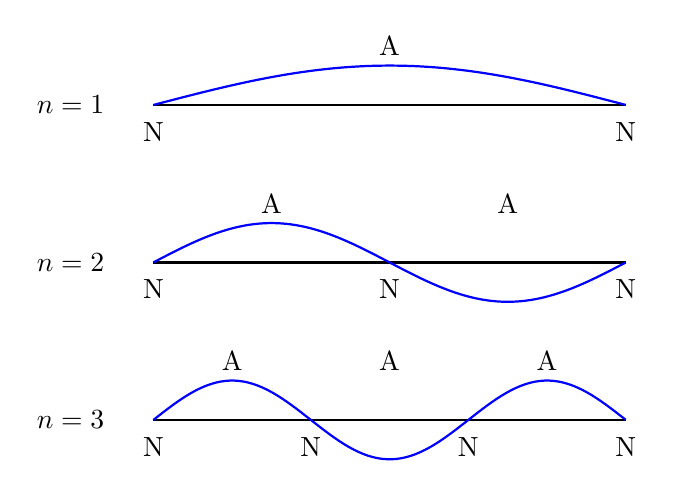
\begin{tikzpicture}[scale=1.0]
% 1st harmonic
\draw[thick] (0,0) -- (6,0);
\draw[thick,blue,domain=0:6,samples=100] plot (\x, {0.5*sin(180*\x/6)});
\node[below] at (0,-0.1) {N};
\node[below] at (6,-0.1) {N};
\node[above] at (3,0.5) {A};
\node[left] at (-0.5,0) {$n=1$};
% 2nd harmonic
\draw[thick] (0,-2) -- (6,-2);
\draw[thick,blue,domain=0:6,samples=100] plot (\x, {0.5*sin(360*\x/6)-2});
\node[below] at (0,-2.1) {N};
\node[below] at (3,-2.1) {N};
\node[below] at (6,-2.1) {N};
\node[above] at (1.5,-1.5) {A};
\node[above] at (4.5,-1.5) {A};
\node[left] at (-0.5,-2) {$n=2$};
% 3rd harmonic
\draw[thick] (0,-4) -- (6,-4);
\draw[thick,blue,domain=0:6,samples=100] plot (\x, {0.5*sin(540*\x/6)-4});
\node[below] at (0,-4.1) {N};
\node[below] at (2,-4.1) {N};
\node[below] at (4,-4.1) {N};
\node[below] at (6,-4.1) {N};
\node[above] at (1,-3.5) {A};
\node[above] at (3,-3.5) {A};
\node[above] at (5,-3.5) {A};
\node[left] at (-0.5,-4) {$n=3$};
\end{tikzpicture}
\end{center}

Key features:
\begin{itemize}
\item 1st harmonic: 2 nodes (both ends), 1 antinode (centre).
\item 2nd harmonic: 3 nodes (both ends + centre), 2 antinodes.
\item 3rd harmonic: 4 nodes (both ends + two interior), 3 antinodes.
\end{itemize}

%% (d) Doppler effect [4 marks]
\item

\textbf{(i)} Source approaching: using $f' = f\dfrac{v}{v - v_s}$ \fromsheet{} (stationary observer, source approaching $\Rightarrow$ denominator uses minus sign): \markstep{1}

$f' = 800\times\frac{340}{340 - 30} = 800\times\frac{340}{310}$

\finalanswer{$f' = 800\times 1.0968 = 877\;\text{Hz}$} \markstep{1}

\textbf{(ii)} Source receding: using $f' = f\dfrac{v}{v + v_s}$ \fromsheet{} (stationary observer, source receding $\Rightarrow$ denominator uses plus sign): \markstep{1}

$f' = 800\times\frac{340}{340 + 30} = 800\times\frac{340}{370}$

\finalanswer{$f' = 800\times 0.9189 = 735\;\text{Hz}$} \markstep{1}

\textit{Note:} The approaching frequency (877~Hz) is higher than the emitted frequency, and the receding frequency (735~Hz) is lower, as expected.

\end{parts}

\newpage

% ---- SOLUTION C4: QUANTUM PHYSICS (15 marks) ----
\question{15}

\noindent\textbf{Basic Dirac Notation and Spin Measurements}

\begin{parts}

%% (a) Normalisation and S_z measurement [3 marks]
\item

\textbf{(i)} The normalisation condition requires $\braket{\psi}{\psi} = 1$: \recalled

$\braket{\psi}{\psi} = \left|\frac{3}{5}\right|^2 + \left|\frac{4}{5}\right|^2 = \frac{9}{25} + \frac{16}{25} = \frac{25}{25} = 1 \quad\checkmark$

\finalanswer{The state is normalised since $|3/5|^2 + |4/5|^2 = 9/25 + 16/25 = 1$.} \markstep{1}

\textbf{(ii)} The state $\ket{\psi} = \frac{3}{5}\ket{\!\uparrow_z} + \frac{4}{5}\ket{\!\downarrow_z}$ is already expressed in the $S_z$ eigenbasis.

By the Born rule \recalled:
\begin{itemize}
\item $S_z = +\hbar/2$ (spin up): probability $= |3/5|^2 = 9/25 = 0.36$
\item $S_z = -\hbar/2$ (spin down): probability $= |4/5|^2 = 16/25 = 0.64$
\end{itemize}

\finalanswer{$P(S_z = +\hbar/2) = 9/25$; \quad $P(S_z = -\hbar/2) = 16/25$.} \markstep{2}

%% (b) Change to x-basis [4 marks]
\item From the formula sheet: \fromsheet

$\ket{\!\uparrow_x} = \frac{1}{\sqrt{2}}\bigl(\ket{\!\uparrow_z} + \ket{\!\downarrow_z}\bigr), \qquad \ket{\!\downarrow_x} = \frac{1}{\sqrt{2}}\bigl(\ket{\!\uparrow_z} - \ket{\!\downarrow_z}\bigr)$

Inverting these relations (add and subtract): \markstep{1}

$\ket{\!\uparrow_z} = \frac{1}{\sqrt{2}}\bigl(\ket{\!\uparrow_x} + \ket{\!\downarrow_x}\bigr), \qquad \ket{\!\downarrow_z} = \frac{1}{\sqrt{2}}\bigl(\ket{\!\uparrow_x} - \ket{\!\downarrow_x}\bigr)$

\markstep{1}

Substituting into $\ket{\psi} = \frac{3}{5}\ket{\!\uparrow_z} + \frac{4}{5}\ket{\!\downarrow_z}$:

$\ket{\psi} = \frac{3}{5}\cdot\frac{1}{\sqrt{2}}\bigl(\ket{\!\uparrow_x} + \ket{\!\downarrow_x}\bigr) + \frac{4}{5}\cdot\frac{1}{\sqrt{2}}\bigl(\ket{\!\uparrow_x} - \ket{\!\downarrow_x}\bigr)$

$= \frac{1}{5\sqrt{2}}\Bigl[(3+4)\ket{\!\uparrow_x} + (3-4)\ket{\!\downarrow_x}\Bigr]$

\finalanswer{$\ket{\psi} = \frac{7}{5\sqrt{2}}\ket{\!\uparrow_x} - \frac{1}{5\sqrt{2}}\ket{\!\downarrow_x}$} \markstep{1}

Probability of measuring $S_x = +\hbar/2$:

$P(S_x = +\hbar/2) = \left|\frac{7}{5\sqrt{2}}\right|^2 = \frac{49}{50}$

\finalanswer{$P(S_x = +\hbar/2) = 49/50 = 0.98$} \markstep{1}

\textit{Check:} $P(S_x = -\hbar/2) = |{-1}/(5\sqrt{2})|^2 = 1/50$. Sum $= 49/50 + 1/50 = 1$ \checkmark

%% (c) Operator analysis [4 marks]
\item

\textbf{(i)} The operator $\hat{A} = \ketbra{\!\uparrow}{\uparrow\!} - \ketbra{\!\downarrow}{\downarrow\!}$.

The matrix elements are: $A_{11} = \bra{\!\uparrow}\hat{A}\ket{\!\uparrow} = 1$, $A_{12} = \bra{\!\uparrow}\hat{A}\ket{\!\downarrow} = 0$, $A_{21} = \bra{\!\downarrow}\hat{A}\ket{\!\uparrow} = 0$, $A_{22} = \bra{\!\downarrow}\hat{A}\ket{\!\downarrow} = -1$.

\finalanswer{$\hat{A} \leftrightarrow \begin{pmatrix} 1 & 0 \\ 0 & -1 \end{pmatrix} = \sigma_z$}

This is the Pauli $z$-matrix. \markstep{1}

\textbf{(ii)} Since the matrix is already diagonal, the eigenvalues and eigenvectors can be read off directly:

\finalanswer{Eigenvalue $+1$ with eigenvector $\ket{\!\uparrow_z} = \begin{pmatrix}1\\0\end{pmatrix}$; \quad Eigenvalue $-1$ with eigenvector $\ket{\!\downarrow_z} = \begin{pmatrix}0\\1\end{pmatrix}$.} \markstep{2}

\textbf{(iii)} $\hat{A}$ is Hermitian. The matrix $\begin{pmatrix}1&0\\0&-1\end{pmatrix}$ is real and symmetric, so its conjugate transpose equals itself:

$\hat{A}^\dagger = \begin{pmatrix}1&0\\0&-1\end{pmatrix}^* {}^T = \begin{pmatrix}1&0\\0&-1\end{pmatrix} = \hat{A}$

\finalanswer{Yes, $\hat{A}$ is Hermitian since $\hat{A}^\dagger = \hat{A}$ (equivalently, the matrix is real and symmetric).} \markstep{1}

%% (d) Eigenstate identification and expectation value [4 marks]
\item The state is $\ket{\psi} = \frac{1}{\sqrt{2}}\bigl(\ket{\!\uparrow_z} + \ket{\!\downarrow_z}\bigr)$.

From the formula sheet: \fromsheet

$\ket{\!\uparrow_x} = \frac{1}{\sqrt{2}}\bigl(\ket{\!\uparrow_z} + \ket{\!\downarrow_z}\bigr)$

Therefore $\ket{\psi} = \ket{\!\uparrow_x}$.

\finalanswer{$\ket{\psi} = \ket{\!\uparrow_x}$, which is an eigenstate of $S_x$.} \markstep{1}

$S_x\ket{\!\uparrow_x} = +\frac{\hbar}{2}\ket{\!\uparrow_x}$

\finalanswer{The eigenvalue is $+\hbar/2$.} \markstep{1}

For the expectation value of $S_z$ on this state: \recalled

$\expect{S_z} = \bra{\psi}S_z\ket{\psi}$

Since $\ket{\psi} = \frac{1}{\sqrt{2}}\ket{\!\uparrow_z} + \frac{1}{\sqrt{2}}\ket{\!\downarrow_z}$, and $S_z = \frac{\hbar}{2}\bigl(\ketbra{\!\uparrow}{\uparrow\!} - \ketbra{\!\downarrow}{\downarrow\!}\bigr)$ \fromsheet: \markstep{1}

$\expect{S_z} = \frac{\hbar}{2}\left(\left|\frac{1}{\sqrt{2}}\right|^2 - \left|\frac{1}{\sqrt{2}}\right|^2\right) = \frac{\hbar}{2}\left(\frac{1}{2} - \frac{1}{2}\right)$

\finalanswer{$\expect{S_z} = 0$} \markstep{1}

This makes physical sense: the state has equal probability of being measured as spin-up or spin-down in the $z$-direction, so the average is zero.

\end{parts}

\end{document}
